\section{Affine $n$-Space and Algebraic Sets}

\begin{definition}
    Let $k$ be a field. We define  \textbf{affine $n$-space} over $k$ to be the
    cartesian product  $\A^n(k) = \underbrace{k \times \dots \times
    k}_{n\text{-times}}$. If the field $k$ is understood, we write  $\A^n$. We
    call the elements of  $\A^(k)$ \textbf{affine points}. We call $\A^1(k)$ and
    $\A^2(k)$ the \textbf{affine line} and \textbf{affine plane} over $k$,
    respectively.
\end{definition}

\begin{definition}
    Let $k$ be a field, and let  $f \in k[x_1, \dots, x_n]$. We call an affine
    point $P \in \A^n(k)$ a \textbf{zero}, or \textbf{root} of $f$ if $f(P)=0$,
    where $f(P)$ is understood to be $f(a_1, \dots, a_n)$, where $P=(a_1, \dots,
    a_n)$. We call the set of zeros of $f$, $V(f)$ the \textbf{hypersurface}
    defined by $f$. We call hypersurfaces in  $\A^2(k)$ \textbf{affine plane
    curves}. If $\deg{f}=1$, we call $V(f)$ a \textbf{hyperplane}. We call
    hypersurfaces in $\A^1(k)$ \textbf{lines}.
\end{definition}

\begin{example}\label{example_2.1}
    The following curves in figure \ref{figure_1.1} define algebraic sets.
    \begin{figure}[h]
        \centering
        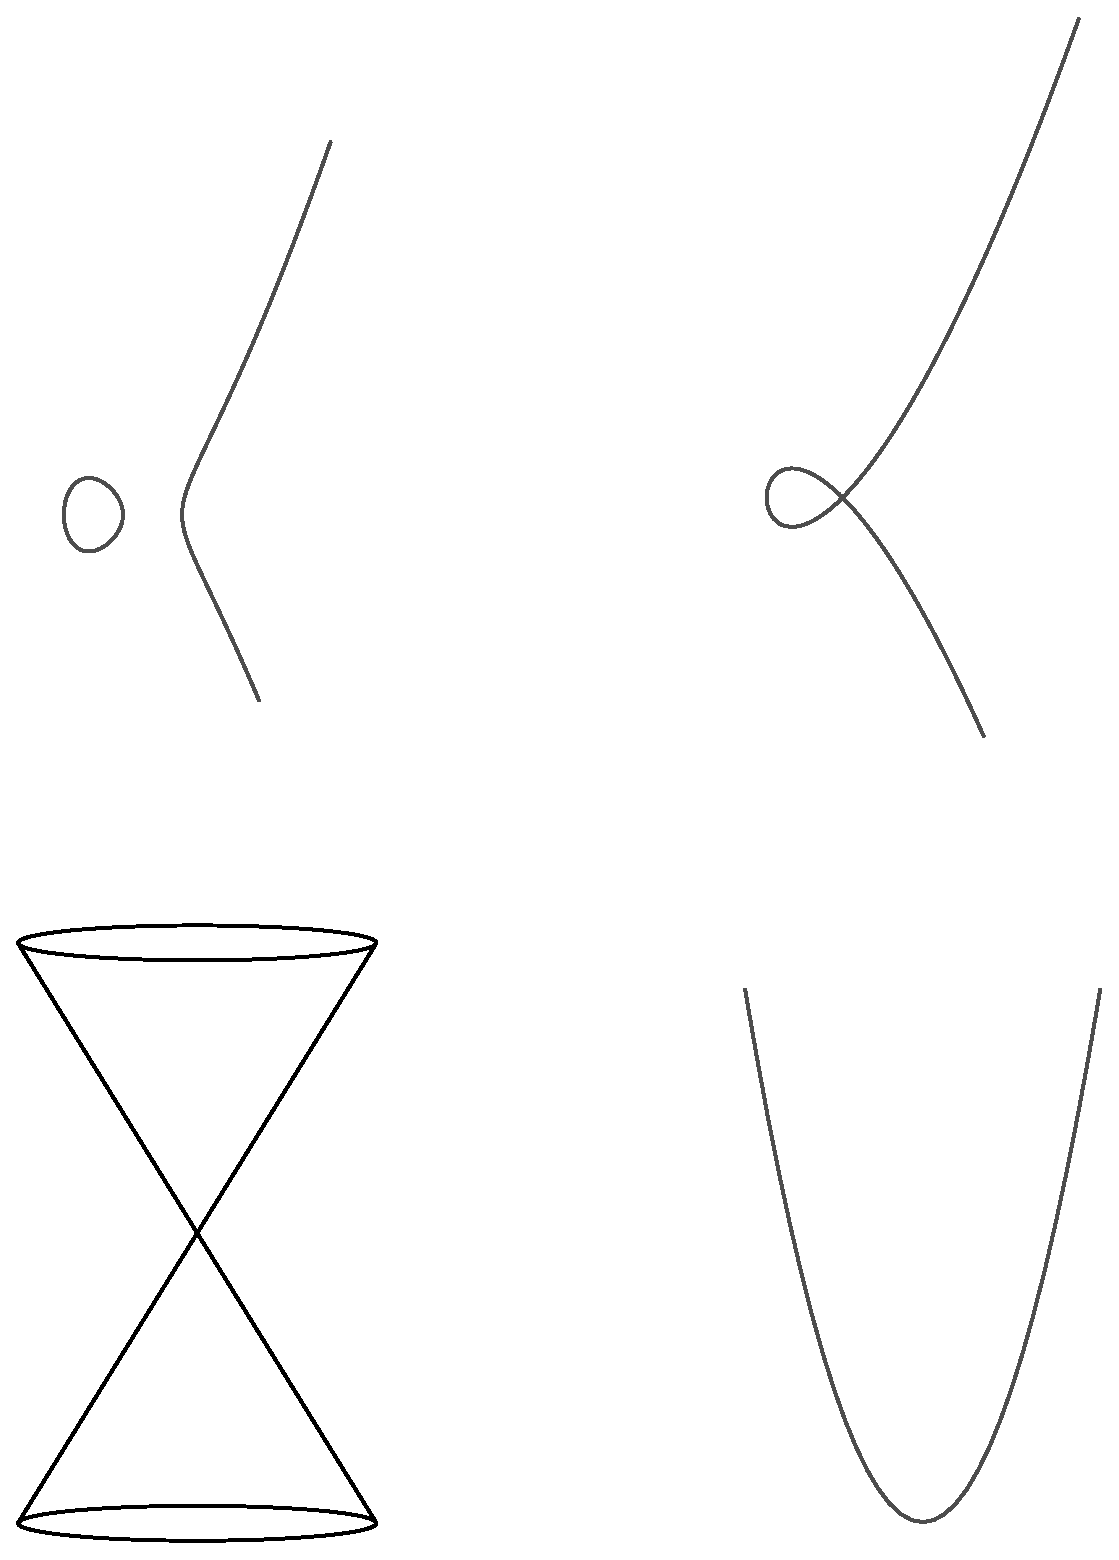
\includegraphics[scale=0.5]{Figures/Chapter1/hyperplanes.eps}
        \caption{Affine Algebraic Sets in $\A^2(\R)$ and $\A^3(\R)$.}
        \label{figure_1.1}
    \end{figure}
\end{example}

\begin{definition}
    Let $k$ be a field, and $S$ any set of polynomials in $k[x_1, \dots, x_n]$.
    We define the \textbf{set of zeros} of $S$ to be the set  $V(S)=\{P \in
    \A^n(k) : f(P)=0 \text{ for all } f \in S\}$. We call a subset $X$ of
    $\A^n(k)$ an \textbf{affine algebraic set} if $X=V(S)$ for some set $S$ of
    polynomials.
\end{definition}

\begin{lemma}\label{1.2.1}
    The following are true for any field $k$.
    \begin{enumerate}
        \item[(1)] If $\af$ is an ideal in $k=[x_1, \dots, x_n]$ generated by a
            set $S \subseteq k[x_1, \dots, x_n]$, then $V(\af)=V(S)$.

        \item[(2)] If $\{\af_\a\}$ is a collection of ideals of $k[x_1, \dots,
            x_n]$, then
            \begin{equation*}
                V\Big{(} \bigcup{\af_\a} \Big{)}=\bigcap{V(\af_\a)}
            \end{equation*}

        \item[(3)] If $\af \subseteq \bf$ are ideals, then  $V(\bf) \subseteq
            V(\af)$.

        \item[(4)] If $f,g \in k[x_1, \dots, x_n]$, then $V(fg)=V(f) \cup V(g)$.

        \item[(5)] $V(0)=\A^n(k)$ and $V(1)=\emptyset$.
    \end{enumerate}
\end{lemma}
\begin{proof}
    First, let $S$ be a set of polynomials in  $k[x_1, \dots, x_n]$. Let
    $\af=(S)$ the ideal generated by $S$. Then if  $f \in S$ is a polynomia,  $f
    \in I$. Then if $P \in \A^n$ is a zero of $f$ in $S$, it is a zero of $f$ in
     $\af$, hence  $V(S) \subseteq V(\af)$. Conversely, we have that if $f \in
     \af$, then by suppostion, $f(x_1, \dots, x_n)=f_1(x_1, \dots,
     x_n)+\dots+f_n(x_1, \dots, x_n)+\dots$. Now, if $f(P)=0$ in $I$, then we
     have $f_i(P)=0$ for every $i$. This makes $f(P)=0$ in $S$, so that  $V(\af)
     \subseteq V(S)$.

     Now, consider the collection $\{\af_\a\}$ of ideals in $k[x_1, \dots,
     x_n]$. Let $P \in V(\bigcup{\af_\a})$. Then for every $f \in
     \bigcup{\af_\a}$, $f(P)=0$ for each $\a$. So that $P \in
     \bigcap{V(\af_\a)}$. Again, on the otherhand, if $P \in
     \bigcap{V(\af_\a)}$, $P \in V(\af_\a)$ for all $\a$ so that  $P \in
     V(\bigcup{\af_\a})$.

     Let $\af$ and  $\bf$ ideals in  $k[x_1, \dots, x_n]$, where $\af \subseteq
     \bf$. Let $P \in V(\bf)$. Then for every polynomial $f \in \bf$, $f(P)=0$,
     so that $f(P)=0$ when $f \in \af$, hence  $P \in V(\af)$. This makes
     $V(\bf) \subseteq V(\af)$.

     Consider now the polynomials $f,g \in k[x_1, \dots, x_n]$. Certainly if $P
     \in V(fg)$ it is a root of $fg$; ie.e.  $fg(P)=0$. This makes $f(P)=0$ or
     $g(P)=0$ so that $V(fg) \subseteq V(f) \cup V(g)$. On the otherhand if $P$
     is a root of $f$, or a root of $g$, it is a root of  $fg$ making  $V(f)
     \cup V(f) \subseteq V(fg)$, and equality is established.

     Finally, observe that the zero polynomial $0(x_1, \dots, x_n)$ has all its
     coefficients $0$, so that any point $P \in \A^n$ is a zero. This makes
     $V(0)=\A^n$. Likewise, the constant polynomial $1(x_1, \dots, x_n)$ has its
     $0$-th coefficient $1$ so that it has not points  $P \in \A^n$ as roots.
     That is  $V(1)=\emptyset$.
\end{proof}
\begin{corollary}
    Finite unions of algebraic sets are algebraic.
\end{corollary}

\begin{example}\label{example_1.2}
    \begin{enumerate}
        \item[(1)] Let $k$ be a field, and consider  $\A^1(k)$. Let $f \in k[x]$
           be a polynomial of degree $n$. Then $f$ has at most $n$ roots in $k$.
           Now, if  $\af$ is an ideal in $k$, since $k$ is a PID, we also get
           $\af=(f)$ for some $f \in k[x]$. That is $|V(\af)| \leq n$, and so
           any algebraic set in $\A^1(k)$ is necessarily finite, except,
           possibly $\A^1(k)$.

       \item[(2)] Let $k$ be a finite field with  $p^m$ elements, where  $p,m
           \in \Z^+$ and $p$ is prime. Then $k$ is the splitting field of the
           polynomial $f(x_n)=x_n^{p^m}-x_n$ over the finite field $\F_p$.
           Suppose then that there is no set $S$ of polynomials in $k[x_1,
           \dots, x_n]$ for which $X=V(S)$, for some $X \in \A^n(k)$. Choose
           then a point $P \in X$ and a polynomial $g \in S$. Then we have
           $g(x_1, \dots,x_n)=g_1(\tilde{X})x_n+\dots+g_n(\tilde{X})x_n$. Notice
           that if $P$ is a root of $f$; i.e. $P \in V(f)$; i.e. $P^{p^m}-P=0$,
           then since $P^{p^m}-P$ is a generator for $k$ as a multiplicative
           group, it generates $S$. That is, $S$ must contain the point $P$ as a
           root for $g$, notice  $P^{p^m}=P$ so that
           $g(P)=g_1(P)P+\dots+g_n(P)P=0$ in $k$. This contradicts that $X \neq
           V(S)$. This makes every set of $\A^n(k)$ algebraic for any finite
           field.

       \item[(3)] By the corollory to lemma \ref{1.2.1}, we have that finite
           unions of algebraic sets are algebraic. Now, consider the field $\Q$,
           and let $f_q(x)=x+\frac{q}{2}$ in $\Q[x]$. We have that there are $X
           \subseteq \A^1(\Q)$ algebraic, ini where $X=V(f_q)$. Notice however,
           that the polynomial
           \begin{equation*}
               f(x)=\prod_{q \in \Q}{f_q(x)}
           \end{equation*}
           has no roots in $\Q$, as that would imply that for some  $n \in
           \Z^+$,  $\sqrt[n]{2} \in \Q$. That is, there is no $X \subseteq
           \A^1(\Q)$ for which $X=V(\prod{f_q})=\bigcup{V(f_q)}$. In general,
           the countable union of algebraic sets need not be algebraic.
    \end{enumerate}
\end{example}

\begin{example}\label{example_1.3}
    \begin{enumerate}
        \item[(1)] Let $k$ be a field, and $X=\{(t,t^2,t^3) \in \A^3(k) : t \in
            k\}$. If $k$ is finite, this is algebraic. Suppose that $k$ is
            infinite, and consider the polynomial
            $f(x_1,x_2,x_3)=x_1+x_2^2+x_3^3$. Notice that the point $0 \in X$ is
            a root of $f$, and that if $P$ is a root of  $f$, then  $P \in X$.
            That is, $X=V(f)$ making $X$ algebraic.

        \item[(2)] Let $X=\{(\cos{t},\sin{t}) \in \A^2(\R) : t \in \R\}$.
            Consider the polynomial $f(x,y)=x^2+y^2-1$. Since we have that
            $\cos^2{t}+\sin^2{t}=1$, $X=V(f)$ and $X$ is algebraic.

        \item[(3)] Let $X=\{(r,\sin{t}) \in \A^2(\R) : r=\sin{t}, t \in \R \}$.
            Consider the polynomial $f(x,y)=x-y$. Then $X=V(f)$.
    \end{enumerate}
\end{example}

\begin{example}\label{example_1.4}
    The following sets are not algebraic.
    \begin{enumerate}
        \item[(1)] $X=\{(x,y) \in \A^2(\R) : y=\sin{x}\}$.

        \item[(2)] $X=\{(z,w) \in \A^2(\C) : |z|^2+|w|^2=1\}$, where
            $|x+iy|^2=x^2+y^2$ for all $x,y \in \R$.

        \item[(3)] $X=\{(\cos{t}, \sin{t}, t) \in \A^3(\R) : t \in \R\}$.
    \end{enumerate}
\end{example}
